\section{Introduction}
\label{sec:introduction}

Monitoring plant biodiversity at scale is essential for understanding ecosystem health, tracking the effects of climate change, and informing conservation policy. Traditionally, vegetation surveys require expert botanists to visit field sites, place standardised quadrats (typically 50$\times$50\,cm sampling frames), and manually identify every plant species visible within the frame. This process is labour-intensive, difficult to scale, and constrained by the availability of trained taxonomists~\cite{joly2024overview}.

The PlantCLEF 2026 challenge~\cite{plantclef2026} seeks to automate this task by framing it as a multi-label classification problem: given a high-resolution photograph of a vegetation quadrat, predict the set of all plant species present. The challenge draws from a taxonomy of approximately 7,800 candidate species, and submissions are evaluated using a macro-averaged F1 score computed 
per quadrat image and then averaged across transects:
\[
  \frac{1}{N}\sum_{i=1}^{N}\!\left(\frac{1}{T_i}
  \sum_{j=1}^{T_i}\mathrm{F1}^{j}\right),
\]
where $N$ is the number of transects, $T_i$ is the number of quadrats 
in transect $i$, and $\mathrm{F1}^{j} = \frac{2 \cdot P_j \cdot R_j}{P_j + R_j}$ 
is the per-image F1 score, with $P_j$ and $R_j$ the precision and 
recall over the predicted species set for quadrat $j$. Averaging first 
within transects then across them prevents high-density sampling sites 
from dominating the final score.

A central difficulty of this challenge is the \emph{domain shift} between the available training data and the target test data. The training set consists of over one million single-plant images from the PlantCLEF 2024 corpus, each depicting an individual specimen with a single species label (Figure~\ref{fig:train_grid}). In contrast, the test images are dense, complex vegetation scenes where multiple species overlap, occlude one another, and appear at varying scales and growth stages (Figure~\ref{fig:quadrats}). Models trained exclusively on isolated specimens tend to perform poorly when confronted with these multi-species scenes, as they have never encountered the visual complexity of real-world vegetation during training.

\begin{figure*}[h]
  \centering
  \resizebox{0.92\linewidth}{!}{% Training-image grid — 6 PlantCLEF~2024 single-plant images in a
% single row. Filenames are content hashes from the PC24 distribution
% and are intentionally omitted from the figure body; species names
% (when known) belong in the host caption.
%
% Required host preamble:
%   \usepackage{graphicx}
%   \usepackage{tikz}

\begin{tikzpicture}[
  every node/.style={inner sep=0pt, outer sep=0pt},
]

\def\cellw{27mm}
\def\cellh{27mm}
\def\colsep{1.5mm}

\node                                       (t1) at (0, 0) {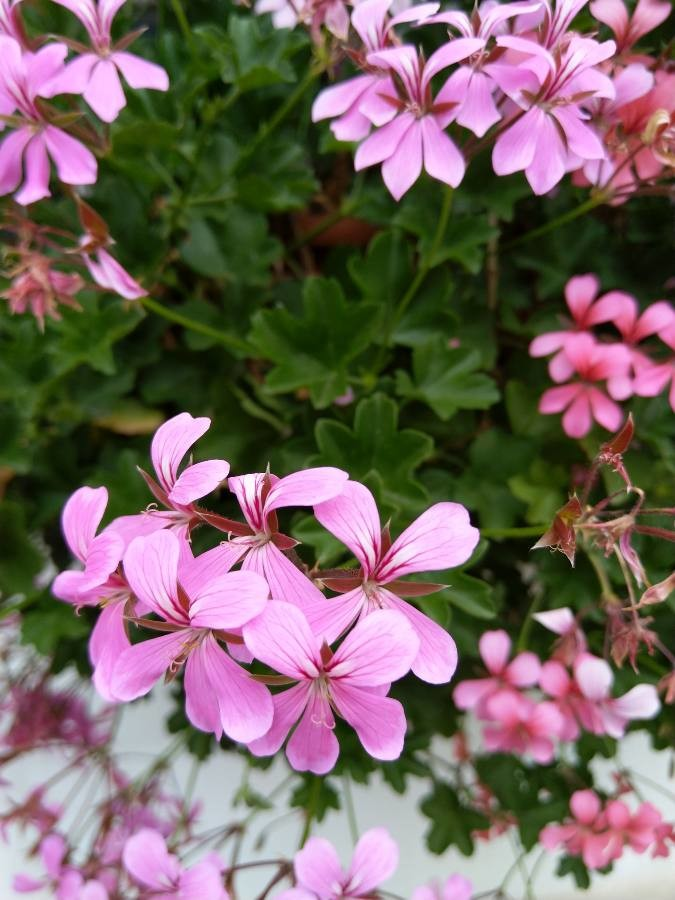
\includegraphics[width=\cellw, height=\cellh, keepaspectratio=false]{images/train/0b4007a0ea47ce9a04625baca25ce8b31eaafb44.jpg}};
\node[right=\colsep of t1.east, anchor=west](t2)            {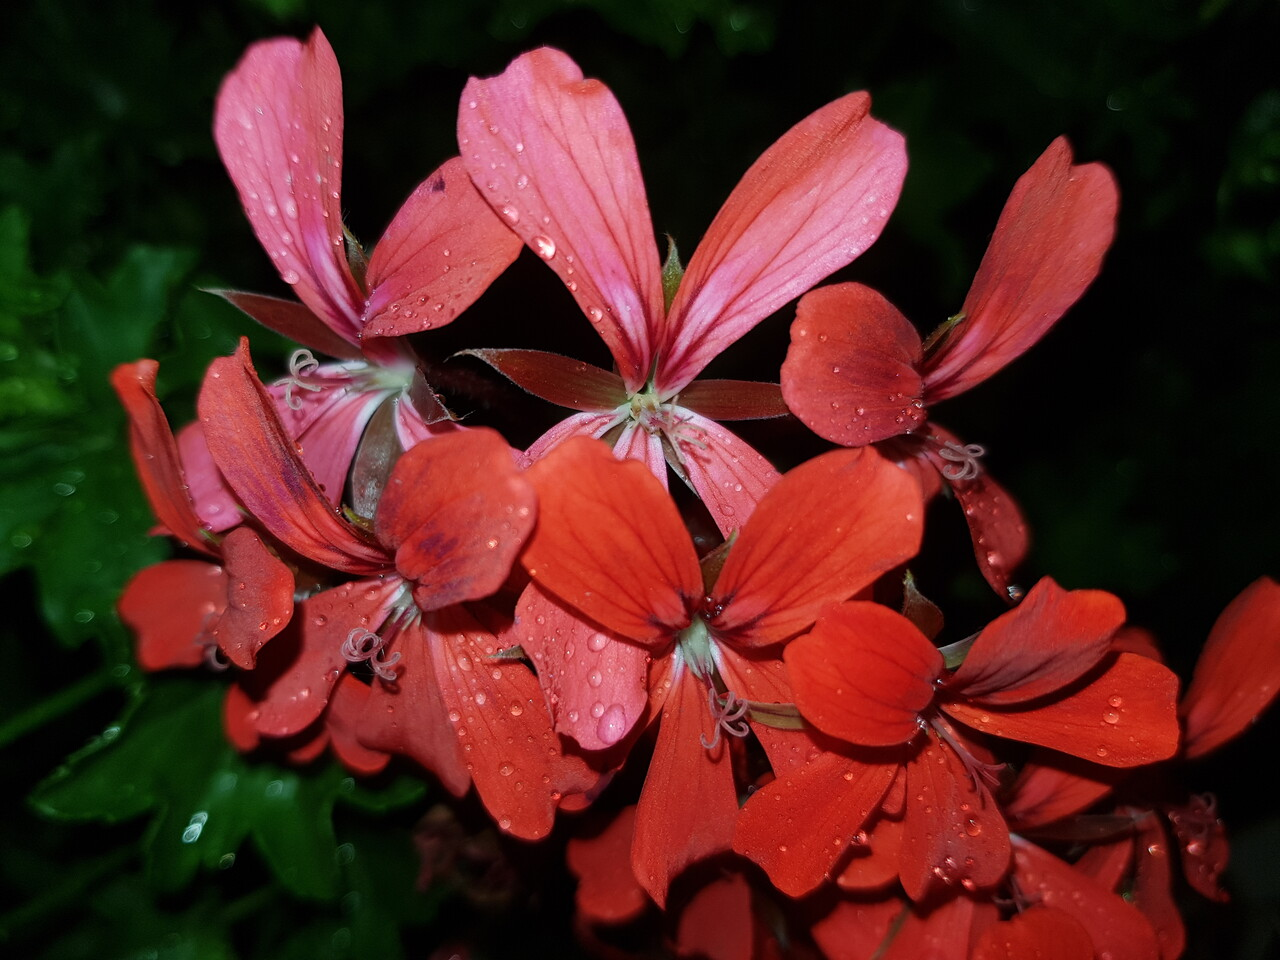
\includegraphics[width=\cellw, height=\cellh, keepaspectratio=false]{images/train/0b5296be0cd6e68cf46f7331edbc54ae600a0f1d.jpg}};
\node[right=\colsep of t2.east, anchor=west](t3)            {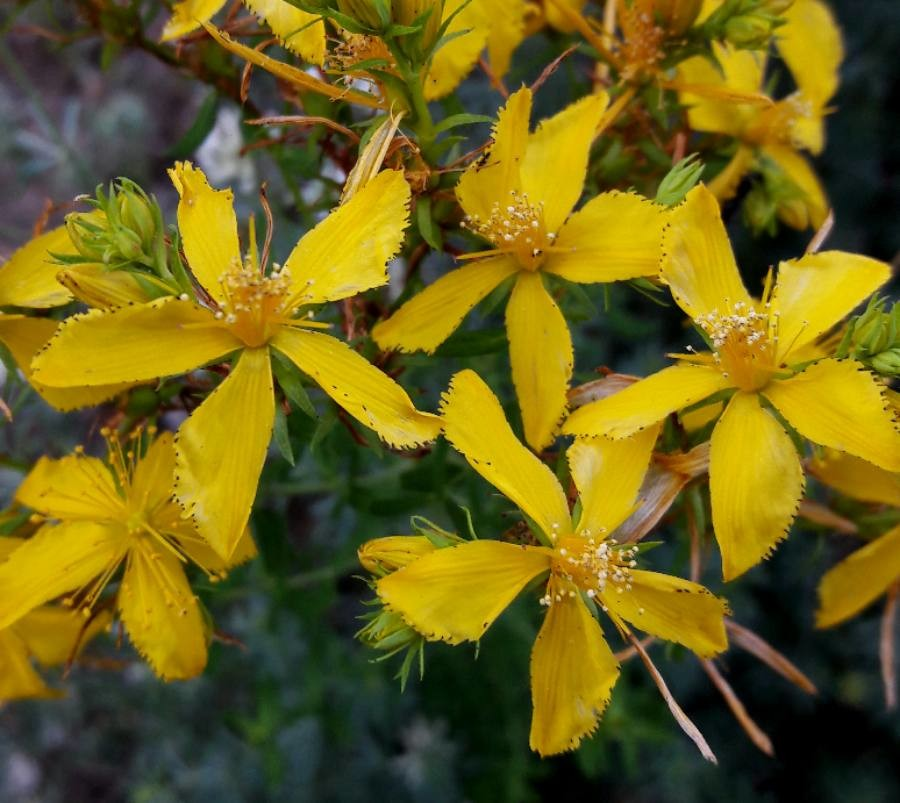
\includegraphics[width=\cellw, height=\cellh, keepaspectratio=false]{images/train/0c5ab5fd302458218691c7833a97688793a7466f.jpg}};
\node[right=\colsep of t3.east, anchor=west](t4)            {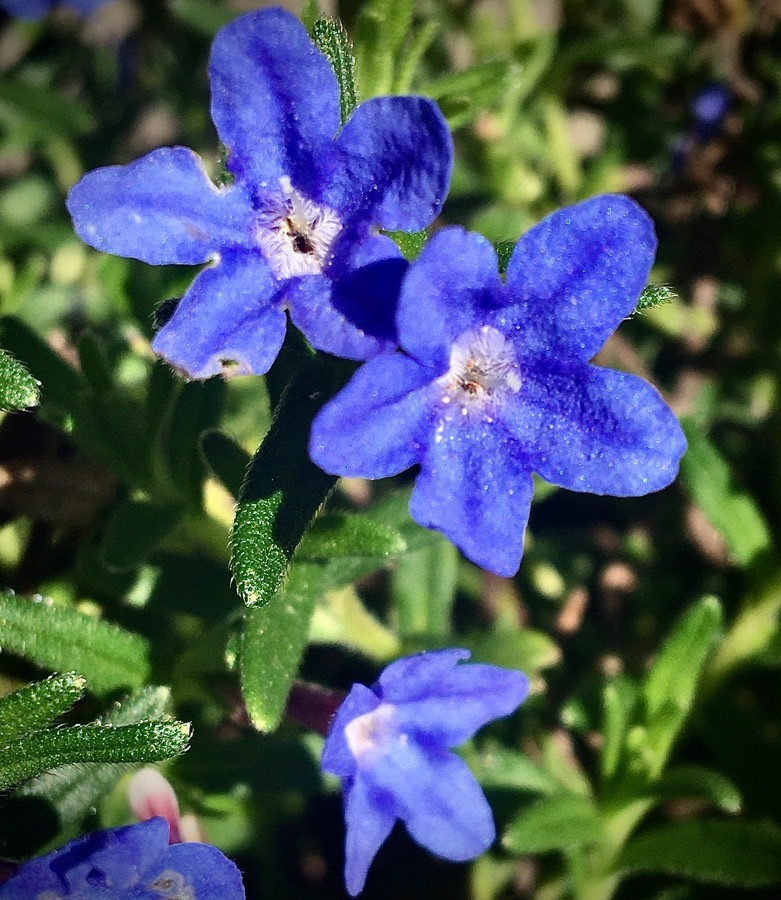
\includegraphics[width=\cellw, height=\cellh, keepaspectratio=false]{images/train/3f2b6248fa328d486b33b4f77f65d6b18b74c5c6.jpg}};
\node[right=\colsep of t4.east, anchor=west](t5)            {
\includegraphics[width=\cellw, height=\cellh, keepaspectratio=false]{images/train/9cf6b7997a95b2bab8d840e70397b98dc8321106.jpg}};
\node[right=\colsep of t5.east, anchor=west](t6)            {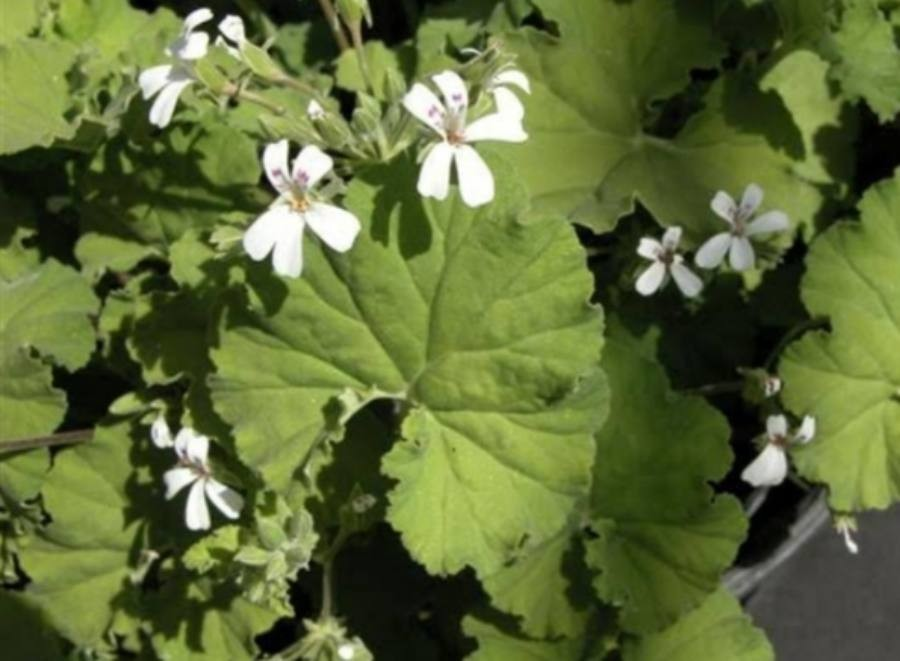
\includegraphics[width=\cellw, height=\cellh, keepaspectratio=false]{images/train/fe3131163544feb319ec6754b79ca33007177e95.jpg}};

\end{tikzpicture}
}
  \caption{Six representative single-plant training images from the PlantCLEF~2024 corpus. Each image carries a single species label and was contributed through the Pl@ntNet citizen-science pipeline. Shooting style is intentionally varied (close-up macro, half-body, full-plant in habitat) and lighting / background are uncontrolled.}
  \label{fig:train_grid}
\end{figure*}

\begin{figure*}[t]
  \centering
  \resizebox{0.92\linewidth}{!}{% Quadrat-grid figure — 6 test-set quadrats in a single row.
% Each cell carries an abbreviated transect-code label above the image
% (the full filenames live in the host caption).
%
% Required host preamble:
%   \usepackage{graphicx}
%   \usepackage{tikz}

\begin{tikzpicture}[
  every node/.style={inner sep=0pt, outer sep=0pt},
  label/.style={font=\sffamily\scriptsize, text=black!70, align=center},
]

\def\cellw{27mm}
\def\cellh{27mm}
\def\colsep{1.5mm}

% Six cells in a single row. Labels are the transect prefix so they fit
% within the narrow cell; the full filename for each is given in the
% host caption.
\node[label]                                       (l1) at (0,                              0) {CBN-PdlC};
\node[below=0.6mm of l1]                           (i1)                                       {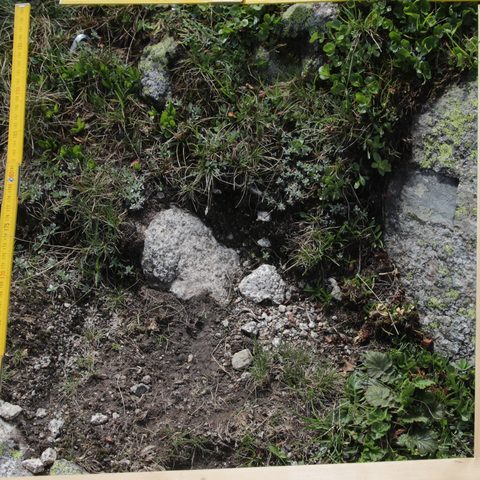
\includegraphics[width=\cellw, height=\cellh, keepaspectratio=false]{images/quadrats/CBN-PdlC-A1-20130807.jpg}};

\node[label, right=\colsep of l1.east, anchor=west](l2) {CBN-Pla};
\node[below=0.6mm of l2]                           (i2) {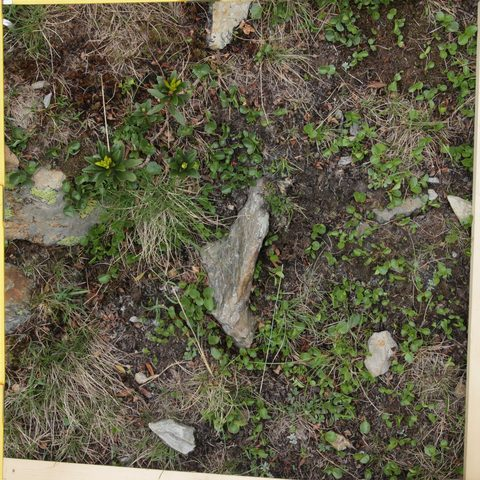
\includegraphics[width=\cellw, height=\cellh, keepaspectratio=false]{images/quadrats/CBN-Pla-A1-20130808.jpg}};

\node[label, right=\colsep of l2.east, anchor=west](l3) {GUARDEN};
\node[below=0.6mm of l3]                           (i3) {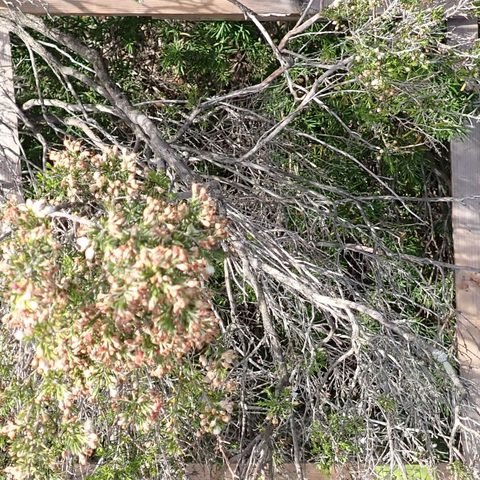
\includegraphics[width=\cellw, height=\cellh, keepaspectratio=false]{images/quadrats/GUARDEN-CBNMed-10-1-16-34-20240429.jpg}};

\node[label, right=\colsep of l3.east, anchor=west](l4) {LISAH-JAS};
\node[below=0.6mm of l4]                           (i4) {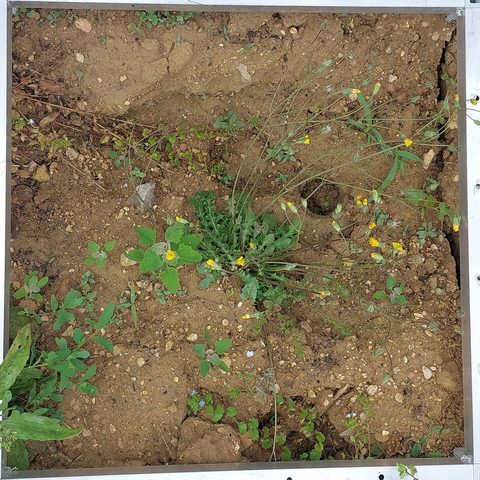
\includegraphics[width=\cellw, height=\cellh, keepaspectratio=false]{images/quadrats/LISAH-JAS-0-1-20220505.jpg}};

\node[label, right=\colsep of l4.east, anchor=west](l5) {OPTMix};
\node[below=0.6mm of l5]                           (i5) {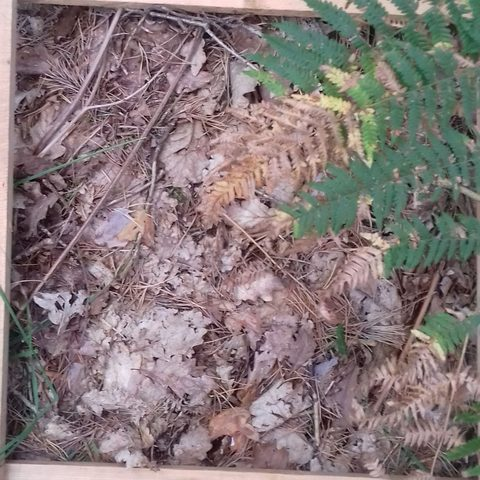
\includegraphics[width=\cellw, height=\cellh, keepaspectratio=false]{images/quadrats/OPTMix-0108-P1-312-20231006.jpg}};

\node[label, right=\colsep of l5.east, anchor=west](l6) {RNNB};
\node[below=0.6mm of l6]                           (i6) {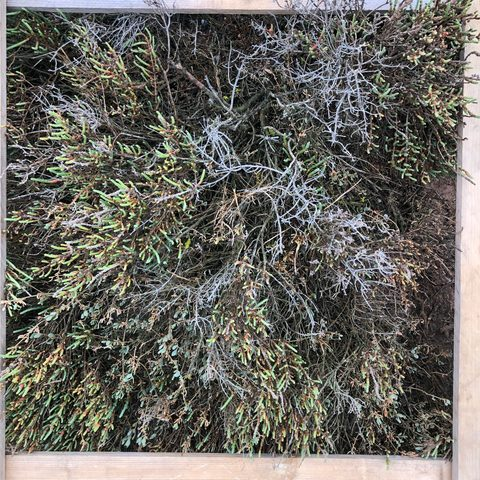
\includegraphics[width=\cellw, height=\cellh, keepaspectratio=false]{images/quadrats/RNNB-1-1-20230512.jpg}};

\end{tikzpicture}
}
  \caption{Six representative quadrats from the PlantCLEF 2026 test set, illustrating the breadth of within-set domain variation. Filenames (left to right): \texttt{CBN-PdlC-A1-20130807}, \texttt{CBN-Pla-A1-20130808}, \texttt{GUARDEN-CBNMed-10-1-16-34-20240429}, \texttt{LISAH-JAS-0-1-20220505}, \texttt{OPTMix-0108-P1-312-20231006}, \texttt{RNNB-1-1-20230512}. Each filename encodes the transect site and observation date. The quadrats range from dense mid-summer canopies (CBN-PdlC, RNNB) to dry shrub-mat communities (LISAH, GUARDEN) and litter-covered shoulder-season frames (OPTMix). Shooting angle, sampling-frame style (wood, tape, painted line), and illumination all vary across the corpus, compounding the single-plant\,$\to$\,multi-species domain shift seen in Figure~\ref{fig:train_grid}.}
  \label{fig:quadrats}
\end{figure*}

A second major challenge is the \emph{long-tail distribution} of the training data. While common species may have thousands of training images, rare species, which are often the most ecologically important, can have fewer than ten. Standard cross-entropy training causes models to overwhelmingly predict common classes, yielding high micro-accuracy but poor macro-F1.

In this paper, we present the system submitted by the Australian National University (ANU) team. Our approach centres on three key design decisions:

\begin{enumerate}
  \item \textbf{Partial-unfreeze BioCLIP 2.5 with taxonomic regularisation.} BioCLIP~\cite{stevens2024bioclip} is a contrastive vision-language model whose pretraining on TreeOfLife-10M aligns its feature space with the Linnaean taxonomy. Rather than fine-tuning the full backbone (which we show collapses this prior), we unfreeze only the last four transformer blocks of BioCLIP 2.5 ViT-H/14 and attach auxiliary cross-entropy heads at coarser taxonomic levels (genus and family in the final design; an earlier multi-task fine-tune additionally used order and class). The auxiliary losses carry small fixed weights, with coarser levels weighted progressively less, so that they primarily regularise the encoder rather than drive it.
  \item \textbf{Long-tail data rebalancing.} The PlantCLEF 2024 single-plant corpus is heavily skewed: a small number of species exceed one thousand training images while hundreds carry fewer than ten. We attack this primarily by enlarging the training manifest to 2.65 million images with pre-filled genus and family labels for every row. A follow-up experiment additionally capped each species at 500 images to flatten the head of the distribution, but this hurt rather than helped (0.40041 vs.\ 0.41826 public Macro F1), evidence that on this benchmark the marginal value of additional head-class examples is positive when label quality is high, and that flattening the distribution discards information rather than rebalancing it.
  \item \textbf{Tile-level inference with adaptive selection.} At inference we partition each quadrat into a non-overlapping $4{\times}4$ grid of sixteen tiles, forward each tile through the encoder at both $224$ and $336$ pixels, and aggregate the per-tile softmax distributions by per-species mean across both the sixteen tiles and the two resolutions. Class-prior logit adjustment ($\tau{=}0.25$) is then applied, which down-weights common species to counteract the long-tail bias. Final selection is adaptive: we emit every species whose post-adjusted probability exceeds a fixed threshold ($T{=}0.03$), with a floor of two and a ceiling of ten species per quadrat. The dual-resolution ensemble ($224$ and $336$ pixels) lifts the public score by $+0.0066$ over the single-resolution baseline; the adaptive threshold outperforms the best fixed top-$k$ ($k{=}2$) by about $0.007$ Macro F1, and by larger margins for other $k$.
\end{enumerate}

\begin{figure}[t]
  \centering
  \includegraphics[width=0.72\linewidth]{figures/training_pipeline}
  \caption{Training pipeline for the ANU PlantCLEF 2026 submission.
The PlantCLEF 2024 single-plant manifest (2.65M images across 7,806
species) is fed into a partially fine-tuned BioCLIP~2.5 ViT-H/14
in which the lower 28 transformer blocks are frozen to preserve the
Tree-of-Life prior and only the last 4 blocks plus the final layer
norm and projection are unfrozen. Auxiliary cross-entropy heads at
the family, genus, and species levels are attached.}
  \label{fig:training_pipeline}
\end{figure}

The remainder of this paper is organised as follows. Section~\ref{sec:related} reviews related work on plant identification, foundation model adaptation, and multi-label classification. Section~\ref{sec:method} defines the final system top-down, from data and label construction through to the final inference pipeline. Section~\ref{sec:experiments} sets out the evaluation protocol, the baseline ladder, and the experiments that justify each component. Section~\ref{sec:analysis} analyses why the system behaves as it does: the validation/leaderboard decoupling, the head representation geometry, the within-backbone saturation, and the long-tail behaviour. Section~\ref{sec:discussion} discusses limitations and future work, and Section~\ref{sec:conclusion} concludes.
